Esto modifica la altura de la onda.

\[\boxed{
  f(x)=A\sin(x)
}\]

\begin{tikzpicture}
  \begin{axis}[
    xmin=0,xmax=2.2*pi,
    ymin=-3.2,ymax=3.2,
    axis lines=middle,
    xtick={0},
    xtick={pi/2,pi,3*pi/2,2*pi},
    xticklabels={
      $\dfrac{\pi}{2}$,
      $\pi$,
      $\dfrac{3}{2}\pi$,
      $2\pi$
    },
    xticklabel style={anchor=south west},
    ytick={-3,-2,-1,1,2,3},yticklabels={$-3$,$-2$,$-1$,$1$,$2$,$3$}
    ]

    \addplot[color=red,samples=100,domain=0:2*pi,thick]{sin(deg(x))};

    \addplot[color=green,samples=100,domain=0:2*pi,thick]{2*sin(deg(x))};

    \addplot[color=blue,samples=100,domain=0:2*pi,thick]{3*sin(deg(x))};

    \legend{$\sin(x)$, $2\sin(x)$, $3\sin(x)$}
  \end{axis}
\end{tikzpicture}
